%-----------------------------------------------------------------------------------
%	PACKAGES AND OTHER DOCUMENT CONFIGURATIONS
%----------------------------------------------------------------------------------

\documentclass{beamer}


\newcommand{\Var}{\mathrm{Var}}

\newcommand{\Cov}{\mathrm{Cov}}

\newcommand{\plim}{\rightarrow_{p}}

\usepackage{apacite}

\usepackage{amsmath, amsfonts}
\usepackage{graphicx}
\usepackage{pdfpages}
\usepackage{bm}
\usepackage{listings}
\usepackage{multirow,array}
\usepackage{enumerate}
\usepackage{bbm}
\usepackage{subfig}
\usepackage{bbm}
\usepackage{multirow}



\usepackage{amssymb}

\usepackage{mathrsfs}
\usepackage{float}
\usepackage{booktabs}
\usepackage{color}
\usepackage{rotating}
\usepackage{amsthm}
\usepackage{multirow,array}
\usepackage{caption}
\usepackage{url}



\DeclareMathOperator*{\argmax}{arg\,max}
\DeclareMathOperator*{\argmin}{arg\,min}



% Expectation symbol
\newcommand{\E}{\mathrm{E}}
\newcommand{\V}{\mathrm{V}}
\newcommand{\N}{\mathcal{N}}
\newcommand{\R}{\mathbb{R}} 

\setbeamertemplate{navigation symbols}{}
 
\addtobeamertemplate{navigation symbols}{}{%
	\usebeamerfont{footline}%
	\usebeamercolor[blue]{footline}%
	\hspace{1em}%
	\insertframenumber/\inserttotalframenumber
}



%-----------------------------
% title stuff 
%-------------------------

\usepackage[utf8]{inputenc}



%Information to be included in the title page:
\title{Incentive effects of social assistance: A regression discontinuity approach}
\author{Thomas Lemieux and Kevin Milligan}
\institute{Journal of Econometrics}
\date{2007}






%------------------------------------------------------------------------------
%	begin doc
%------------------------------------------------------------------------------

\begin{document}
	


%------------------------------------------------------------------------------
%	frame 
%------------------------------------------------------------------------------
	
	\frame{\titlepage}
	




%------------------------------------------------------------------------------
%	frame 
%------------------------------------------------------------------------------

\begin{frame}
\frametitle{Introduction}

\begin{itemize}
		\setlength{\itemsep}{5mm}
	\item Investigating impact of social assistance programs on employment 
	\item Implement a regression discontinuity approach utilizing discontinuity in social assistance payments in Quebec at age 30
	\item Form a first difference estimator in the regression discontinuity design
	\item They compare their estimates to common difference in difference specifications 
\end{itemize}


\end{frame}


%------------------------------------------------------------------------------
%	frame 
%------------------------------------------------------------------------------

\begin{frame}
\frametitle{Social assistance in Quebec and Canada }

\begin{itemize}
	\setlength{\itemsep}{5mm}
	\item Until 1989 
	\begin{itemize}
		\setlength{\itemsep}{3mm}
		\item Those under 30 received \$185 per month
		\item Those over 30 received \$507 per month
		\item 175\% increase 
	\end{itemize}

\item After 1989 all receive \$507 
\item Benefits are reduced dollar for dollar

\item Basic labor supply model predicts fall in employment 
\begin{itemize}
	\item Don't work and receive benefits
	\item Or, work optimal hours 
	\item Anyone who's utility with the 30 and up benefits now exceeds utility of working will drop out 
\end{itemize}

\end{itemize}
\end{frame}

%------------------------------------------------------------------------------
%	frame 
%------------------------------------------------------------------------------



\begin{frame}
\frametitle{Social assistance in Quebec and Canada}
	\framesubtitle{Graphical representation}
	
	\begin{center}
		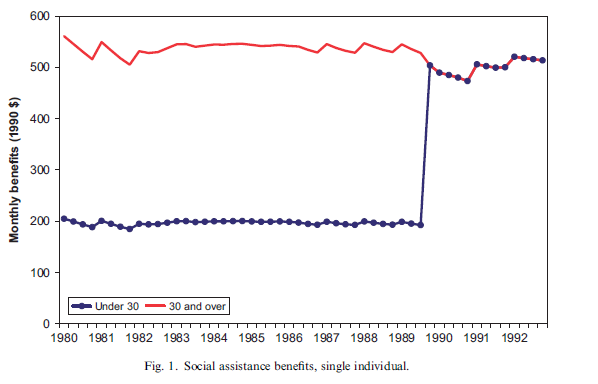
\includegraphics[width=.95\linewidth]{fig_1.PNG}
		
	\end{center}
	
\end{frame}






%------------------------------------------------------------------------------
%	frame 
%------------------------------------------------------------------------------


\begin{frame}
\frametitle{Data and Descriptive Statistics }
\begin{itemize}
	\item 1986, and 1991 census 
	\item Labor force survey (LFS). Used as Time series compliment 
	\item Some questions aked about week prior to survey 
	\begin{itemize}
		\item Employment status 
		\item Hours worked 
		\item Marital status 
	\end{itemize}
	\item Others measure over previous calendar year 
	\begin{itemize}
		\item Income by source 
		\item "Other transfers" is particularly important as it contains social assistance. (85\% of category)
		\item Number of weeks worked in previous year 
	\end{itemize}
\end{itemize}
\end{frame}

%------------------------------------------------------------------------------
%	frame 
%------------------------------------------------------------------------------
\begin{frame}
\frametitle{Data and Descriptive Statistics}
\framesubtitle{Subseting}
\begin{itemize}
	\item Focus on high school dropouts 
	\begin{itemize}
		\item 63\% of claimants are HS Dropouts (59.7\% in their sample)
	\end{itemize}
	\item Respondents without children 
	\begin{itemize}
		\item Having children gets you higher assistance regardless of age 
		\item Excluding this makes it a "sharp" RD 
	\end{itemize}
	\item Men only 
	\begin{itemize}
		\item By 30 many more women have children 
		\item Much lower general employment for High School dropouts among women
	\end{itemize}
	\item Ultimately sample of 3000-1000 HS dropouts without kids  for each age 24-39
\end{itemize}

\end{frame}


%------------------------------------------------------------------------------
%	frame 
%------------------------------------------------------------------------------
\begin{frame}
\frametitle{Data and Descriptive Statistics}
\framesubtitle{LFS Data }

	\begin{center}
	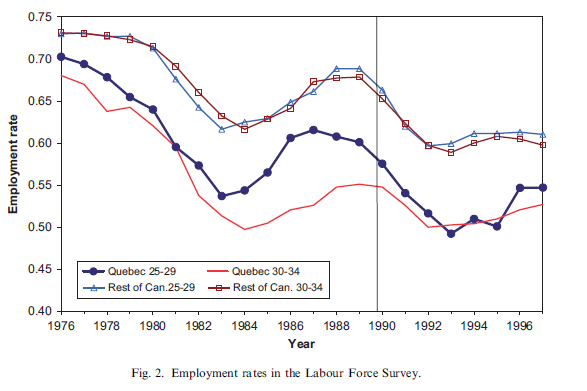
\includegraphics[width=.95\linewidth]{fig_2.PNG}
	
\end{center}


\end{frame}




%------------------------------------------------------------------------------
%	frame 
%------------------------------------------------------------------------------

\begin{frame}
\frametitle{Empirical Approach}

\begin{center}
   \textbf{Individual Specification} 
\end{center}
$$ Y_{ia} = \beta_0 + \beta_1 \textbf{TREAT}_{ia} + \delta(a) + \epsilon_{ia}$$

\begin{itemize}
\item $\delta(\cdot)$ must be smooth
\item Treatment is "sharp" (thanks to subsetting)
\end{itemize}

\begin{center}
	\resizebox{.65\linewidth}{!}{\begin{tabular}{||c | c||} 
			\hline
			Variable & Meaning  \\ [0.5ex] 
			\hline\hline
			$i$ & Individual  \\ 
			\hline 
			$a$ & Age\\ 
			\hline
			$Y$ & Outcome Variable \\
			\hline
			TREAT & 0 if $a < 30$, 1 otherwise\\
			\hline
			$\delta(a)$ & effect of age on outcome variable\\
			\hline
			$\epsilon$ & random noise\\[1ex] 
			\hline
		\end{tabular}
	}
\end{center}

\end{frame}

%------------------------------------------------------------------------------
%	frame 
%------------------------------------------------------------------------------

\begin{frame}
\frametitle{Empirical Approach}

\begin{itemize}
	\setlength{\itemsep}{6mm}
\item Can only observe age at time of survey, so age is discrete 
\item Age specific means are a sufficient statistic, giving an alternative equation 

$$ Y_{a} = \beta_0 + \beta_1 \textbf{TREAT}_{a} + \delta(a) + \epsilon_{a}$$

\item Properly weighting these cells gives the same result as individual regression


\end{itemize}

\end{frame}


%------------------------------------------------------------------------------
%	frame 
%------------------------------------------------------------------------------

\begin{frame}
\frametitle{Empirical Approach}

\begin{itemize}
	\item RD is "fuzzy" for variables measured over previous calendar year 
	\item Assign treatment based on June 1st census day and assumed uniform distribution of birth dates 
	
	$$ TREAT'_i = \begin{cases} 
	0 & if \; a \leq 29, \\
	.170 & if \; a = 30 \\
	.913 & if \; a = 31 \\
	1 & if \; a \geq 32.
	\end{cases}$$
	
	
\end{itemize}

\end{frame}

%------------------------------------------------------------------------------
%	frame 
%------------------------------------------------------------------------------


\begin{frame}
	\frametitle{Empirical Approach}
	\begin{itemize}
		\item Define ERC as employment rate based on reference week of Census 
		\item Define ERL as employment rate based on fraction of weeks worked in last year
		$$ ERC_a = \beta_0 + \beta_1TREAT_a + \delta(a) + \epsilon_a$$
		$$ERL_a = \beta'_0 + \beta'_1TREAT'_a + \delta'(a) + \epsilon'_a$$
		
		\item If we assume $\beta_1 = \beta'_1$ we can get a FD-RD estimator 
		$$ERC_a-ERL_a = (\beta_0 - \beta'_0) + \beta_1(TREAT_a - TREAT'_a) + \theta(a) + (\epsilon_a - \epsilon'_a)$$
		\item This compares employment of same individuals at 29 and 30 
	\end{itemize}
	
	
	
	
\end{frame}


%------------------------------------------------------------------------------
%	frame 
%------------------------------------------------------------------------------

\begin{frame}
\frametitle{Regression Discontinuity Estimates}
\framesubtitle{Graphical Evidence}


	\begin{center}
	\textbf{Employment rate in Census week}
	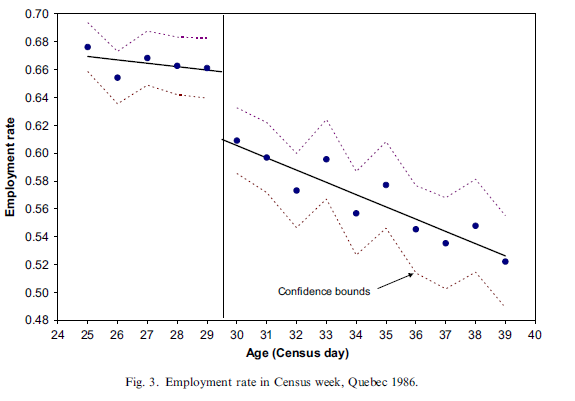
\includegraphics[width=.95\linewidth]{fig_3.PNG}
	
\end{center}

\end{frame}


%------------------------------------------------------------------------------
%	frame 
%------------------------------------------------------------------------------

\begin{frame}
\frametitle{Regression Discontinuity Estimates}
\framesubtitle{Graphical Evidence}

\begin{center}
		\textbf{Employment rate in previous year}
	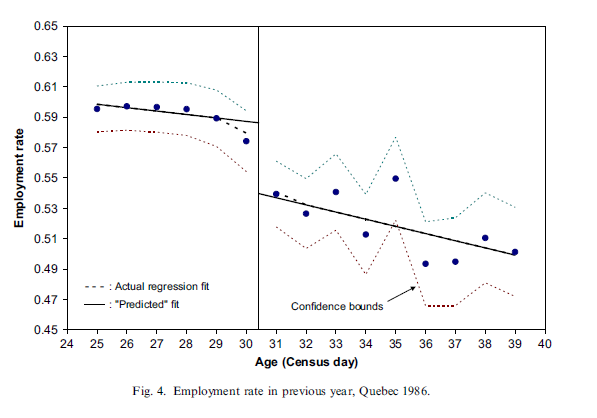
\includegraphics[width=.95\linewidth]{fig_4.PNG}
	
\end{center}

\end{frame}


%------------------------------------------------------------------------------
%	frame 
%------------------------------------------------------------------------------

\begin{frame}
\frametitle{Regression Discontinuity Estimates}
\framesubtitle{Results}

\begin{center}

	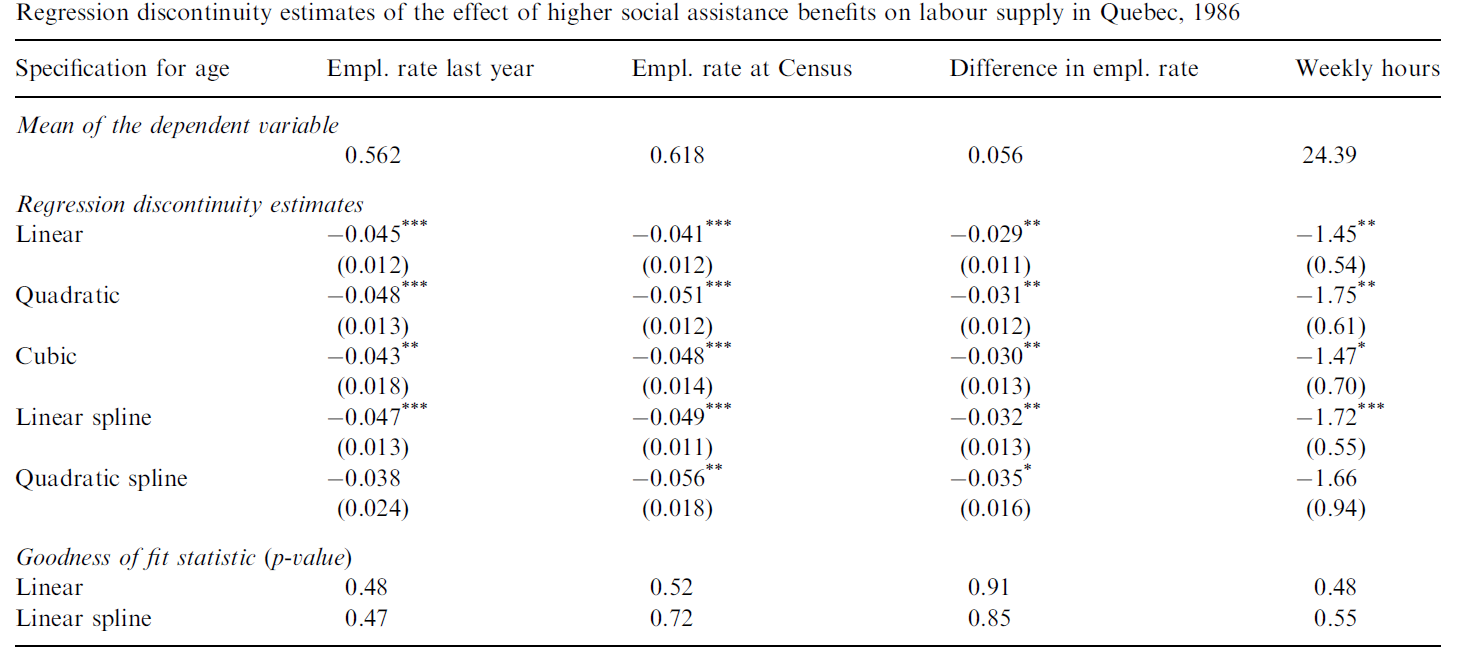
\includegraphics[width=1\linewidth]{table_1.PNG}mnn
	
\end{center}

\end{frame}



%------------------------------------------------------------------------------
%	frame 
%------------------------------------------------------------------------------

\begin{frame}
\frametitle{Regression Discontinuity Estimates}


\begin{center}

	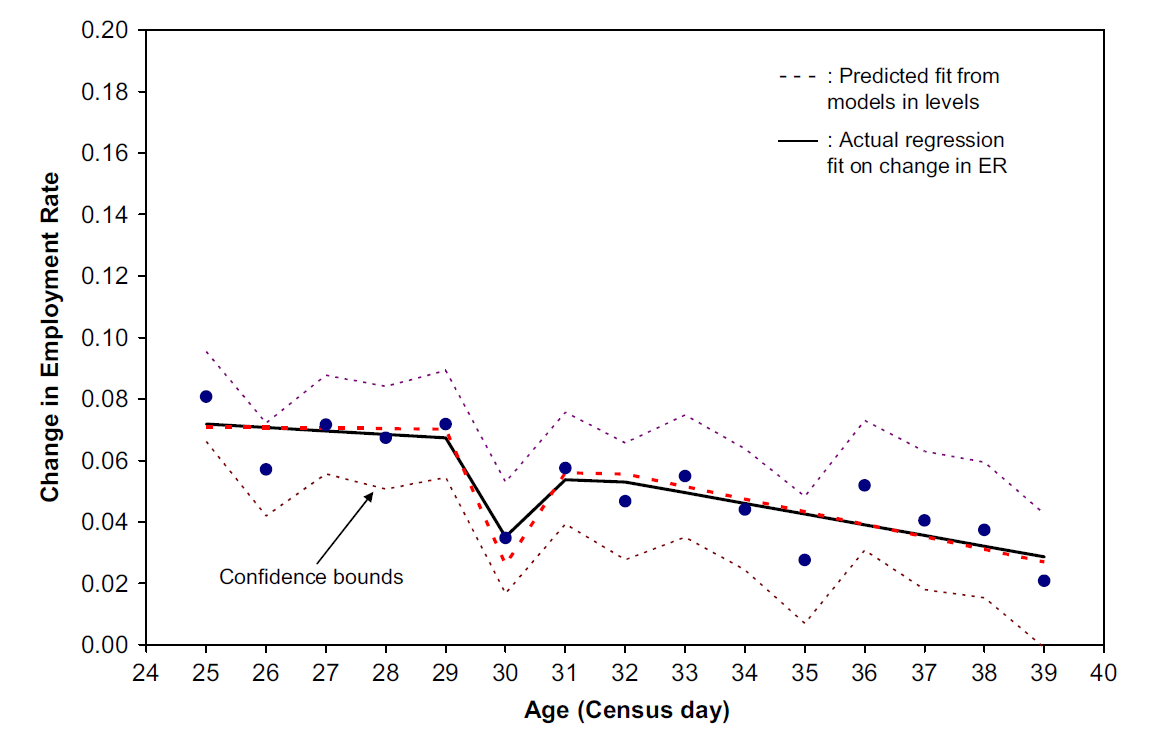
\includegraphics[width=.95\linewidth]{fig_5.PNG}
	
\end{center}

\end{frame}

%------------------------------------------------------------------------------
%	frame 
%------------------------------------------------------------------------------

\begin{frame}
\frametitle{Robustness Checks}
\framesubtitle{Checking Bandwidth}

\begin{center}
	
	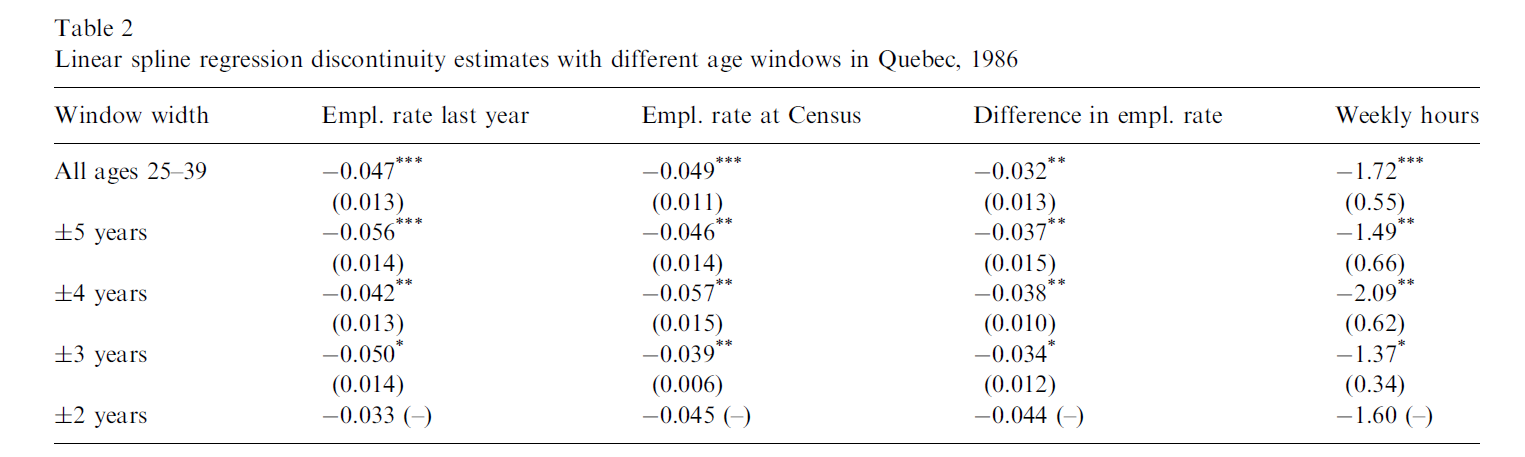
\includegraphics[width=.95\linewidth]{table_2.PNG}
	
\end{center}

\end{frame}


%------------------------------------------------------------------------------
%	frame 
%------------------------------------------------------------------------------

\begin{frame}
\frametitle{Robustness Checks}
\framesubtitle{Falsification tests}

\begin{center}
	
	\includegraphics[width=1\linewidth]{table_3.PNG}
	
\end{center}

\end{frame}

%------------------------------------------------------------------------------
%	frame 
%------------------------------------------------------------------------------

\begin{frame}
\frametitle{Robustness Checks}
\framesubtitle{Other Transfers}

\begin{center}
	
	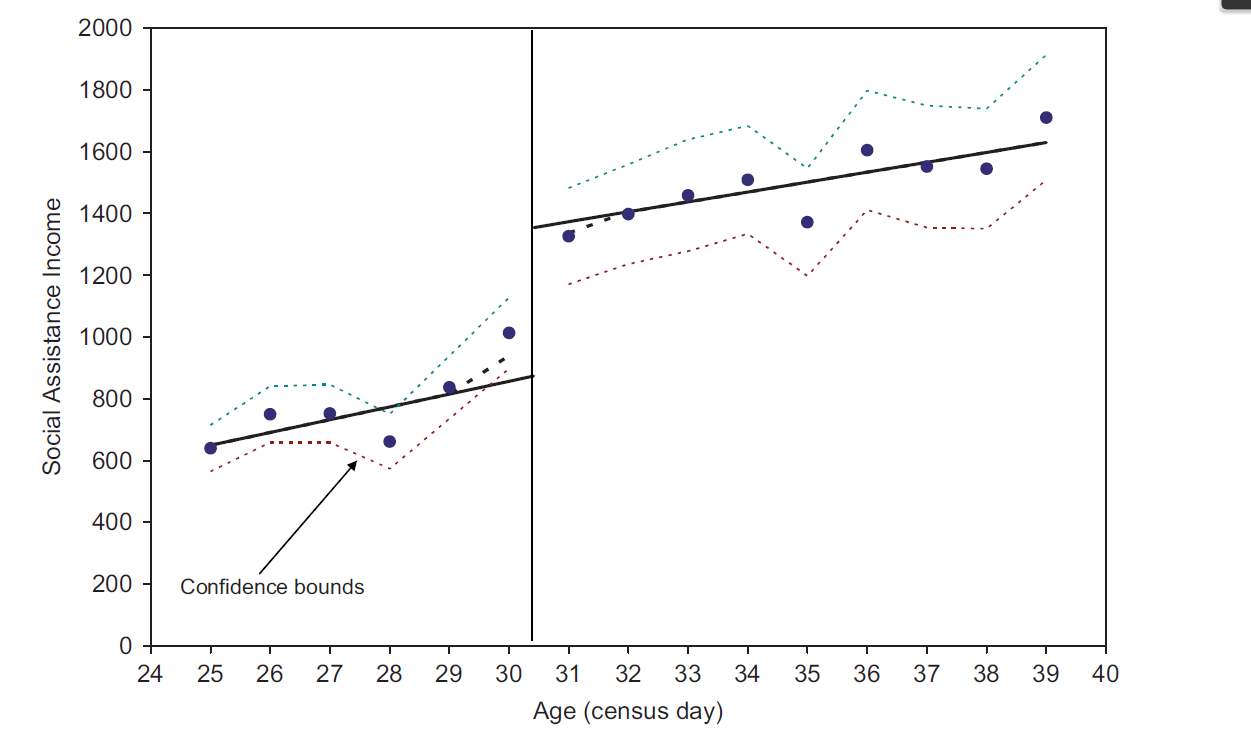
\includegraphics[width=1\linewidth]{fig_6.PNG}
	
\end{center}

\end{frame}



%------------------------------------------------------------------------------
%	frame 
%------------------------------------------------------------------------------

\begin{frame}
\frametitle{Comparing RD and difference-in-differences results}

\begin{center}
	
	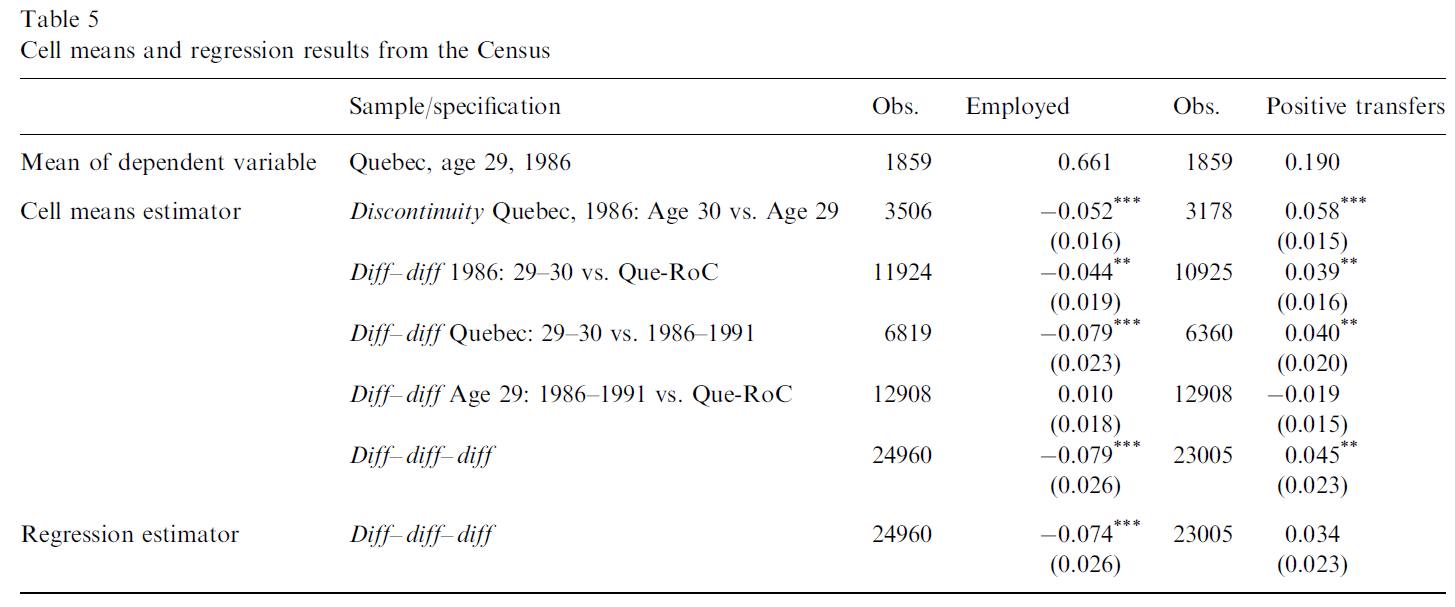
\includegraphics[width=1\linewidth]{table_5.PNG}
	
\end{center}

\end{frame}


%------------------------------------------------------------------------------
%	frame 
%------------------------------------------------------------------------------

\begin{frame}
\frametitle{Comparing RD and difference-in-differences results}

\begin{itemize}
	\item First diff-in-diff is Quebec 29 vs 30 and the rest of Canada 29 vs 30 all in 1986 
	\item Second is using Quebec in 1991 as a control group
	\item Third is Quebec 29 in 2986 vs 1991 against same thing in rest of Canada
	\item diff-diff-diff is 1986 29 to 30 gap in Quebec vs the rest of Canada vs this difference again in 1991
\end{itemize}
\end{frame}


%------------------------------------------------------------------------------
%	frame 
%------------------------------------------------------------------------------

\begin{frame}
\frametitle{Conclusion}
\begin{itemize}
	\item Main finding: “more generous assistance benefits reduces the employment probability of less educated men without dependent children"
	\item Employment rate drops 3-5 \% points with a 175\% increase in benefits 
	\item Identified for men ages 29-30 only
	\item  Only get TOT that might not generalize to other groups 
	\item Difference in difference only works well when using a control group from the same time period
\end{itemize}
\end{frame}


%------------------------------------------------------------------------------
%	frame 
%------------------------------------------------------------------------------

\begin{frame}

\frametitle{The End }

\begin{center}
	
	\begin{Huge}
		\textbf{Thank You}
	\end{Huge}
\end{center}
\end{frame}

%------------------------------------------------
% end doc
%------------------------------------------------
\end{document}
